\section{第六周数值分析实验}
\subsection{Bernstein多项式}
\begin{definition}
	设$f:[0,1]\to\mathbb{R}$,称
	$$
	B_n(f;x)=\sum_{i=0}^{n}f\left(\frac{i}{n}\right)B_i^n(x),x\in[0,1]
	$$
	为$f$的$n$次Bernstein多项式,其中$B_i^n(x)=\binom{n}{i}x^i(1-x)^{n-i}$.
\end{definition}
\lstinputlisting[language=matlab]{day5/bernstein_n.m}
\begin{ex}
	当$f(x)=\cos 2\pi x$时,分别给出$n=3, 5, 7, 9, 10$时的$B_n(f,x)$表达式,并绘制$f(x)$与$B_n(f,x)$的图像.
\end{ex}
\lstinputlisting[language=matlab]{day5/work6.m}
\qa 

\begin{flalign*}
	&B_3(f,x)=\frac{9\,x^2}{2}-\frac{9\,x}{2}+1.&
\end{flalign*}
\begin{flalign*}
	\begin{split}
		B_5(f,x)=&-\frac{17396110258977045\,x^4}{2251799813685248}+\frac{69584441035908185\,x^3}{4503599627370496}\\&-\frac{19232666484692435\,x^2}{4503599627370496}-\frac{3889888508315415\,x}{1125899906842624}+1.
	\end{split}&
\end{flalign*}
\begin{flalign*}
	\begin{split}
		B_7(f,x)=&\frac{7\,x^7}{36028797018963968}+\frac{48511846945173955\,x^6}{18014398509481984}-\frac{291071081671043793\,x^5}{36028797018963968}\\&-\frac{39777928968693195\,x^4}{9007199254740992}+\frac{100417737650160665\,x^3}{4503599627370496}-\frac{22201645688437845\,x^2}{2251799813685248}\\&-\frac{11869558316351393\,x}{4503599627370496}+1.
	\end{split}&
\end{flalign*}
\begin{flalign*}
	\begin{split}
		B_9(f,x)=&-\frac{63\,x^9}{2251799813685248}-\frac{3651501963845295\,x^8}{9007199254740992}+\frac{912875490961461\,x^7}{562949953421312}\\&+\frac{4844390630064489\,x^6}{1125899906842624}-\frac{41846600653847829\,x^5}{2251799813685248}+\frac{21573830928373101\,x^4}{4503599627370496}\\&+\frac{26215294559596821\,x^3}{1125899906842624}-\frac{29056921947987975\,x^2}{2251799813685248}-\frac{18965558858231295\,x}{9007199254740992}+1.
	\end{split}&
\end{flalign*}
\begin{flalign*}
	\begin{split}
		B_{10}(f,x)=&\frac{36617051598889\,x^{10}}{4503599627370496}-\frac{183085257994425\,x^9}{4503599627370496}-\frac{1745013596718105\,x^8}{2251799813685248}\\&+\frac{3764655080427825\,x^7}{1125899906842624}+\frac{16286793569370555\,x^6}{4503599627370496}-\frac{51167254958838837\,x^5}{2251799813685248}\\&+\frac{42639379132365645\,x^4}{4503599627370496}+\frac{25803329789012535\,x^3}{1125899906842624}-\frac{15656499233079345\,x^2}{1125899906842624}\\&-\frac{1075138741208855\,x}{562949953421312}+1.
	\end{split}&
\end{flalign*}

\begin{figure}[H]
	\centering
	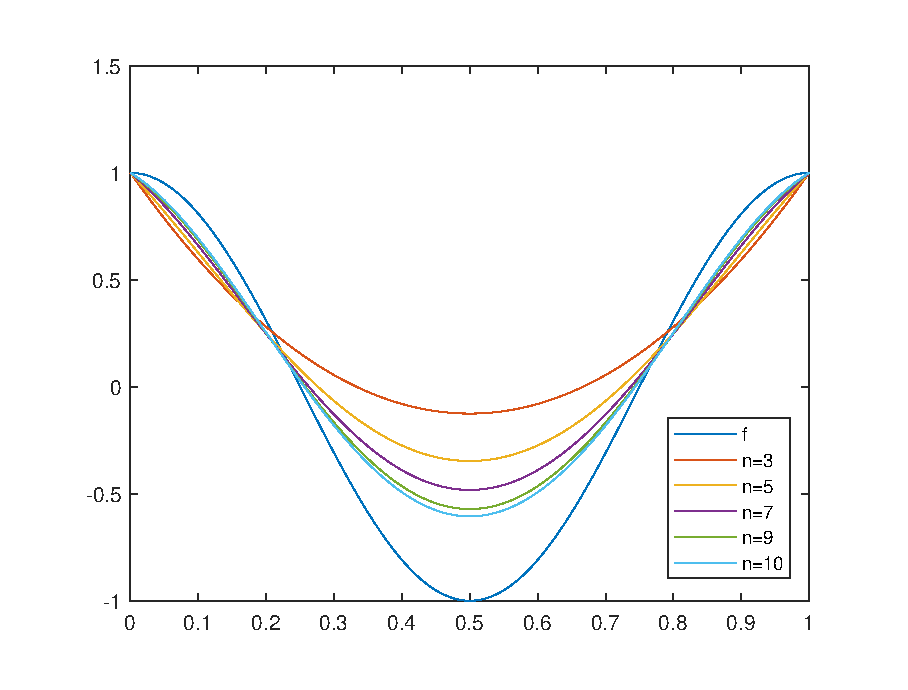
\includegraphics[width = 0.6\linewidth]{day5/fig.eps}
	\caption{Bernstein多项式图像}
\end{figure}